%%
%% This is file `sample-sigconf.tex',
%% generated with the docstrip utility.
%%
%% The original source files were:
%%
%% samples.dtx  (with options: `sigconf')
%% 
%% IMPORTANT NOTICE:
%% 
%% For the copyright see the source file.
%% 
%% Any modified versions of this file must be renamed
%% with new filenames distinct from sample-sigconf.tex.
%% 
%% For distribution of the original source see the terms
%% for copying and modification in the file samples.dtx.
%% 
%% This generated file may be distributed as long as the
%% original source files, as listed above, are part of the
%% same distribution. (The sources need not necessarily be
%% in the same archive or directory.)
%%
%% The first command in your LaTeX source must be the \documentclass command.
\documentclass[sigconf]{acmart}

%%
%% \BibTeX command to typeset BibTeX logo in the docs
\AtBeginDocument{%
  \providecommand\BibTeX{{%
    \normalfont B\kern-0.5em{\scshape i\kern-0.25em b}\kern-0.8em\TeX}}}

%% Rights management information.  This information is sent to you
%% when you complete the rights form.  These commands have SAMPLE
%% values in them; it is your responsibility as an author to replace
%% the commands and values with those provided to you when you
%% complete the rights form.
\setcopyright{acmcopyright}
\copyrightyear{2020}
\acmYear{2020}
\acmDOI{10.1145/3185768.3186313}

%% These commands are for a PROCEEDINGS abstract or paper.
\acmConference[ICPE '20]{ICPE '20: ACM/SPEC International Conference on Performance Engineering}{April 20--24, 2020}{Edmonton, Canada}
\acmBooktitle{ICPE '20: ACM/SPEC International Conference on Performance Engineering,
  April 20--24, 2020, Edmonton, Canada}
\acmPrice{15.00}
\acmISBN{978-1-4503-XXXX-X/18/06}


%%
%% Submission ID.
%% Use this when submitting an article to a sponsored event. You'll
%% receive a unique submission ID from the organizers
%% of the event, and this ID should be used as the parameter to this command.
%%\acmSubmissionID{123-A56-BU3}

%%
%% The majority of ACM publications use numbered citations and
%% references.  The command \citestyle{authoryear} switches to the
%% "author year" style.
%%
%% If you are preparing content for an event
%% sponsored by ACM SIGGRAPH, you must use the "author year" style of
%% citations and references.
%% Uncommenting
%% the next command will enable that style.
%%\citestyle{acmauthoryear}

%%
%% end of the preamble, start of the body of the document source.
\begin{document}

%%
%% The "title" command has an optional parameter,
%% allowing the author to define a "short title" to be used in page headers.
\title{Machine learning to find optimal carbon tax policy to increase investment in low-carbon technologies using agent-based models}

%%
%% The "author" command and its associated commands are used to define
%% the authors and their affiliations.
%% Of note is the shared affiliation of the first two authors, and the
%% "authornote" and "authornotemark" commands
%% used to denote shared contribution to the research.
%\author{Alexander Kell}
%\affiliation{%
%  \department{School of Computing}
%  \institution{Newcastle University}
%  \city{Newcastle upon Tyne}
%  \country{UK}
%}
%\email{a.kell2@newcastle.ac.uk}
%
%\author{A. Stephen McGough}
%\affiliation{%
%  \department{School of Computing}
%  \institution{Newcastle University}
%  \city{Newcastle upon Tyne}
%  \country{UK}
%}
%\email{stephen.mcgough@newcastle.ac.uk}
%
%\author{Matthew Forshaw}
%\affiliation{%
%  \department{School of Computing}
%  \institution{Newcastle University}
%  \city{Newcastle upon Tyne}
%  \country{UK}
%}
%\email{matthew.forshaw@newcastle.ac.uk}
\author{Anonymized}
%%
%% By default, the full list of authors will be used in the page
%% headers. Often, this list is too long, and will overlap
%% other information printed in the page headers. This command allows
%% the author to define a more concise list
%% of authors' names for this purpose.
\renewcommand{\shortauthors}{Kell et al.}

%%
%% The abstract is a short summary of the work to be presented in the
%% article.
\begin{abstract}
 
 Placeholder
 
\end{abstract}

%%
%% The code below is generated by the tool at http://dl.acm.org/ccs.cfm.
%% Please copy and paste the code instead of the example below.
%%


%%
%% Keywords. The author(s) should pick words that accurately describe
%% the work being presented. Separate the keywords with commas.
\keywords{Energy markets, policy, carbon tax, genetic algorithm, optimization}

%% A "teaser" image appears between the author and affiliation
%% information and the body of the document, and typically spans the
%% page.


%%
%% This command processes the author and affiliation and title
%% information and builds the first part of the formatted document.
\maketitle

\section{Introduction}
ACM's consolidated article template, introduced in 2017, provides a
consistent \LaTeX\ style for use across ACM publications, and
incorporates accessibility and metadata-extraction functionality
necessary for future Digital Library endeavors. Numerous ACM and
SIG-specific \LaTeX\ templates have been examined, and their unique
features incorporated into this single new template.

If you are new to publishing with ACM, this document is a valuable
guide to the process of preparing your work for publication. If you
have published with ACM before, this document provides insight and
instruction into more recent changes to the article template.

The ``\verb|acmart|'' document class can be used to prepare articles
for any ACM publication --- conference or journal, and for any stage
of publication, from review to final ``camera-ready'' copy, to the
author's own version, with {\itshape very} few changes to the source.

\section{Literature Review}
As noted in the introduction, the ``\verb|acmart|'' document class can
be used to prepare many different kinds of documentation --- a
double-blind initial submission of a full-length technical paper, a
two-page SIGGRAPH Emerging Technologies abstract, a ``camera-ready''
journal article, a SIGCHI Extended Abstract, and more --- all by
selecting the appropriate {\itshape template style} and {\itshape
  template parameters}.

This document will explain the major features of the document
class. For further information, the {\itshape \LaTeX\ User's Guide} is
available from
\url{https://www.acm.org/publications/proceedings-template}.


\section{Problem Formulation}

Modifying the template --- including but not limited to: adjusting
margins, typeface sizes, line spacing, paragraph and list definitions,
and the use of the \verb|\vspace| command to manually adjust the
vertical spacing between elements of your work --- is not allowed.

{\bfseries Your document will be returned to you for revision if
  modifications are discovered.}

\section{Results}

Here are the results


\begin{figure}
\centering
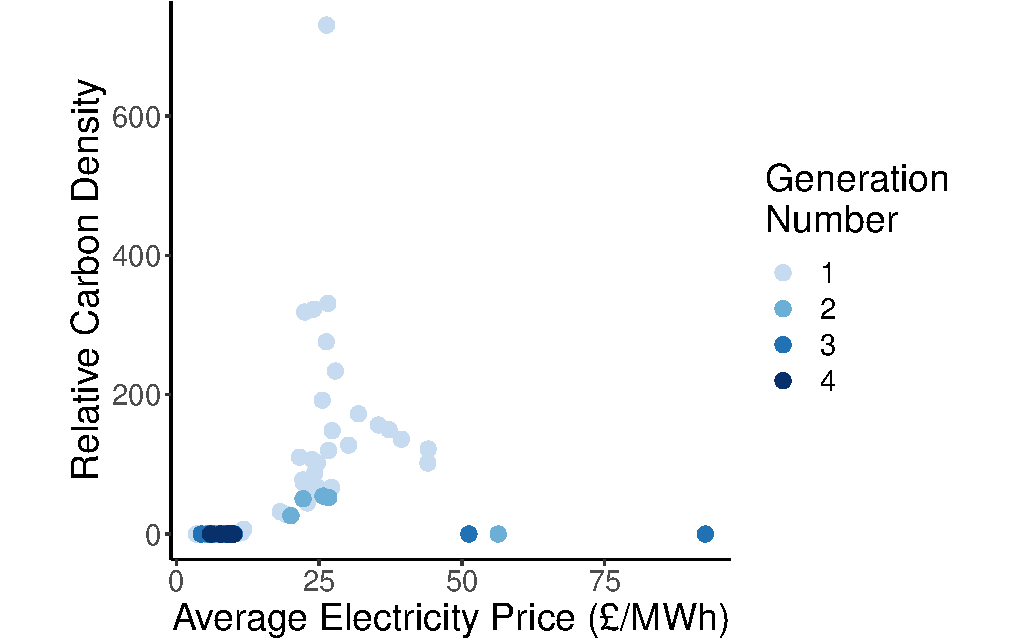
\includegraphics[width=0.49\textwidth]{/Users/b1017579/Documents/PhD/Papers/6-carbon-optimiser/acmart-master/samples/figures/results/free_points/free_points_ga_development.pdf}
\caption{Development of genetic algorithm rewards of average electricity price and relative carbon density in 2035 over time for highest degrees of freedom per year.}
\label{fig:forward_scenario_best_pdcs1}
\end{figure}



\begin{figure}
\centering
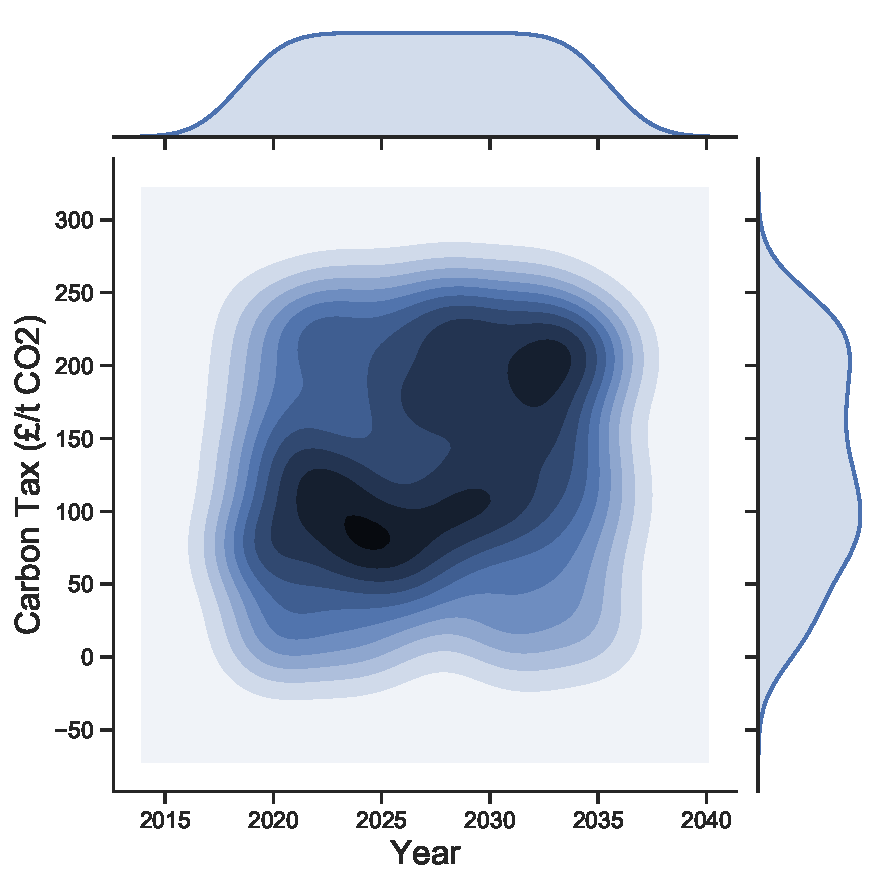
\includegraphics[width=0.49\textwidth]{/Users/b1017579/Documents/PhD/Papers/6-carbon-optimiser/acmart-master/samples/figures/results/free_points/best_heatmap.pdf}
\caption{2D density plot of carbon tax strategies that led to an average electricity price of below \textsterling5/MWh by 2035.}
\label{fig:forward_scenario_best_pdcs}
\end{figure}


\begin{figure}
\centering
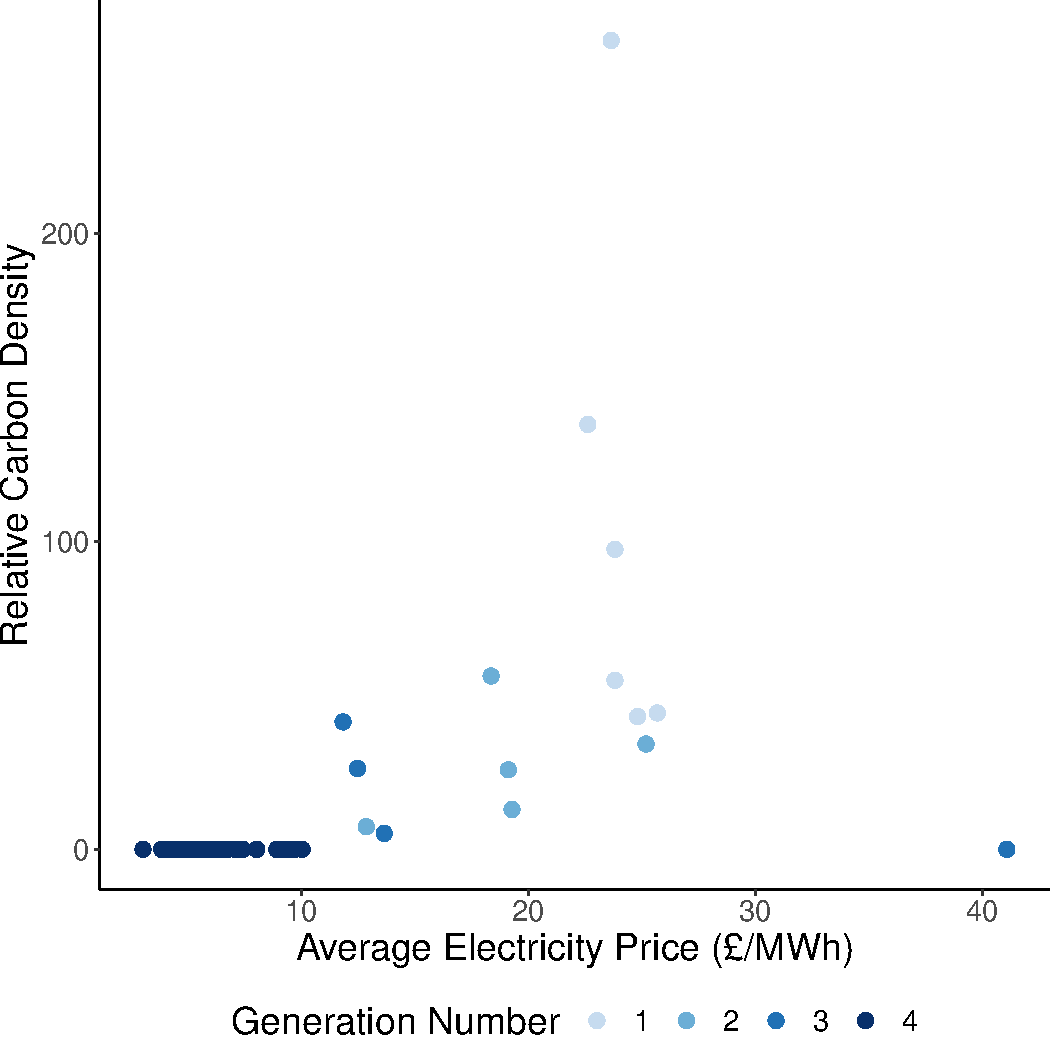
\includegraphics[width=0.49\textwidth]{/Users/b1017579/Documents/PhD/Papers/6-carbon-optimiser/acmart-master/samples/figures/results/linear/linear_ga_development.pdf}
\caption{Development of genetic algorithm rewards of average electricity price and relative carbon density in 2035 over time for linear carbon strategy.}
\label{fig:forward_scenario_best_pdcs}
\end{figure}


\begin{figure}
\centering
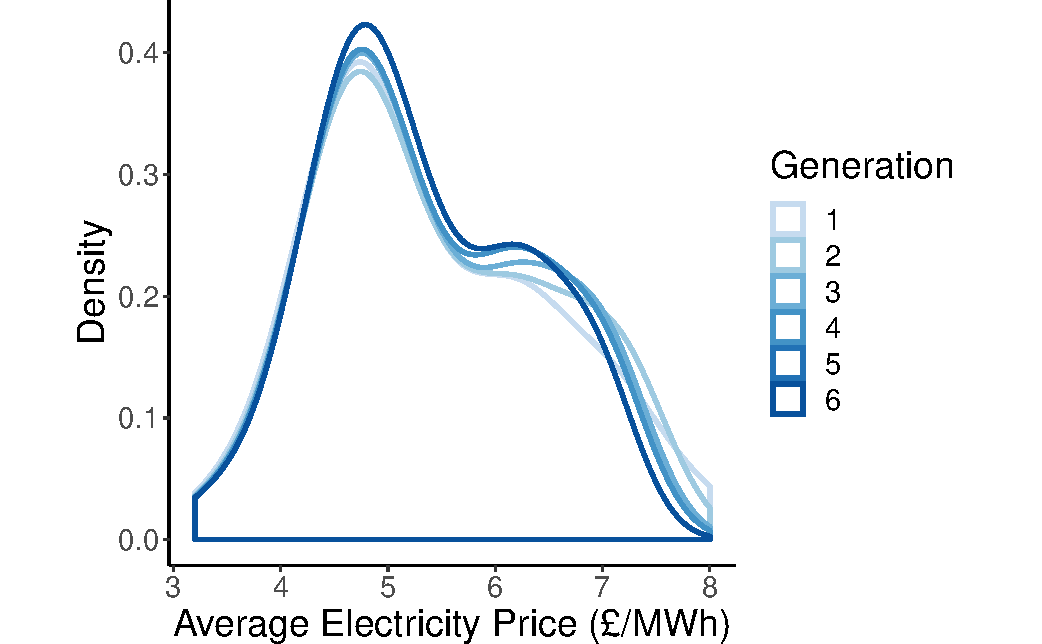
\includegraphics[width=0.49\textwidth,]{/Users/b1017579/Documents/PhD/Papers/6-carbon-optimiser/acmart-master/samples/figures/results/linear/linear_ga_development_distribution.pdf}
\caption{Density plot of average electricity price smaller than \textsterling 8/MWh in 2035 over generation number of genetic algorithm.}
\label{fig:forward_scenario_best_pdcs}
\end{figure}



\begin{figure}
\centering
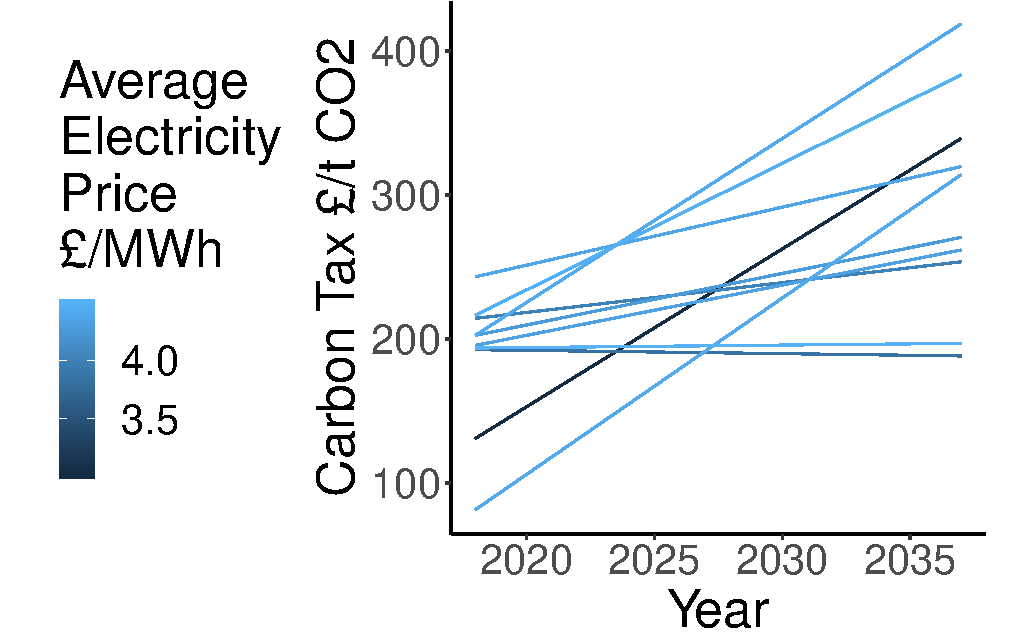
\includegraphics[width=0.49\textwidth,]{/Users/b1017579/Documents/PhD/Papers/6-carbon-optimiser/acmart-master/samples/figures/results/linear/linear_actual_lines.pdf}
\caption{Linear carbon tax strategies visualised with average electricity price smaller than \textsterling 5/MWh.}
\label{fig:forward_scenario_best_pdcs}
\end{figure}



\section{Conclusion}

The title of your work should use capital letters appropriately -
\url{https://capitalizemytitle.com/} has useful rules for
capitalization. Use the {\verb|title|} command to define the title of
your work. If your work has a subtitle, define it with the
{\verb|subtitle|} command.  Do not insert line breaks in your title.

If your title is lengthy, you must define a short version to be used
in the page headers, to prevent overlapping text. The \verb|title|
command has a ``short title'' parameter:
\begin{verbatim}
  \title[short title]{full title}
\end{verbatim}


%\section{Acknowledgments}



\begin{acks}
Anonymized
%This work was supported by the Engineering and Physical Sciences Research Council, Centre for Doctoral Training in Cloud Computing for Big Data [grant number EP/L015358/1].
\end{acks}

%%
%% The next two lines define the bibliography style to be used, and
%% the bibliography file.
\bibliographystyle{ACM-Reference-Format}
\bibliography{sample-base}

%%
%% If your work has an appendix, this is the place to put it.
\appendix


\end{document}
\endinput
%%
%% End of file `sample-sigconf.tex'.
